\section{Audio: Reconocimiento de Voz y Clasificación de Audio}
\label{sec:annex-18}

\subsection{Resumen Ejecutivo}

\texttt{frankenstein\_audio} es la cuarta clase de modelo del conjunto de herramientas. Posee un frontend de audio---bancos de filtros log-mel o un espectrograma crudo, SpecAugment opcional \citep{Park2019} y dos convoluciones con stride 2 que reducen la tasa de tramas $4\times$---y luego ejecuta la misma pila de \texttt{HybridLayer} que el encoder de texto sobre la secuencia de tramas resultante. Como la pila es agnóstica de modalidad, todos los mezcladores de secuencia (incluido el Conformer del Anexo~\ref{sec:annex-17}), normas, estrategias de residual, codificaciones posicionales, optimizadores y bloques de enrutamiento están disponibles sin cambios. La clase soporta dos tareas: \textbf{reconocimiento automático de voz} (\texttt{asr}, con pérdida CTC \citep{Graves2006ctc} o RNN-Transducer \citep{Graves2012}) y \textbf{clasificación de audio} (\texttt{audio\_classification}, entropía cruzada a nivel de clip). El mismo frontend, con \texttt{audio.feature: raw}, acepta señales de sensores multicanales unidimensionales como EEG, EMG o acelerómetro para clasificación.

La receta de referencia es el frontend Conformer de \citet{Gulati2020}: bancos de filtros log-mel de 80 canales con ventana de 25\,ms y salto de 10\,ms, dos convoluciones $3\times3$ con stride 2, una proyección lineal al ancho del modelo y SpecAugment con ancho de frecuencia $F=27$, diez máscaras temporales y una razón máxima de máscara temporal $p_S = 0.05$. Los tres tamaños de referencia (S/M/L) se reproducen en la Tabla~\ref{tab:audio-sizes}.

\subsection{La Clase de Modelo \texttt{frankenstein\_audio}}

\begin{figure}[H]
\centering
\fitfigure{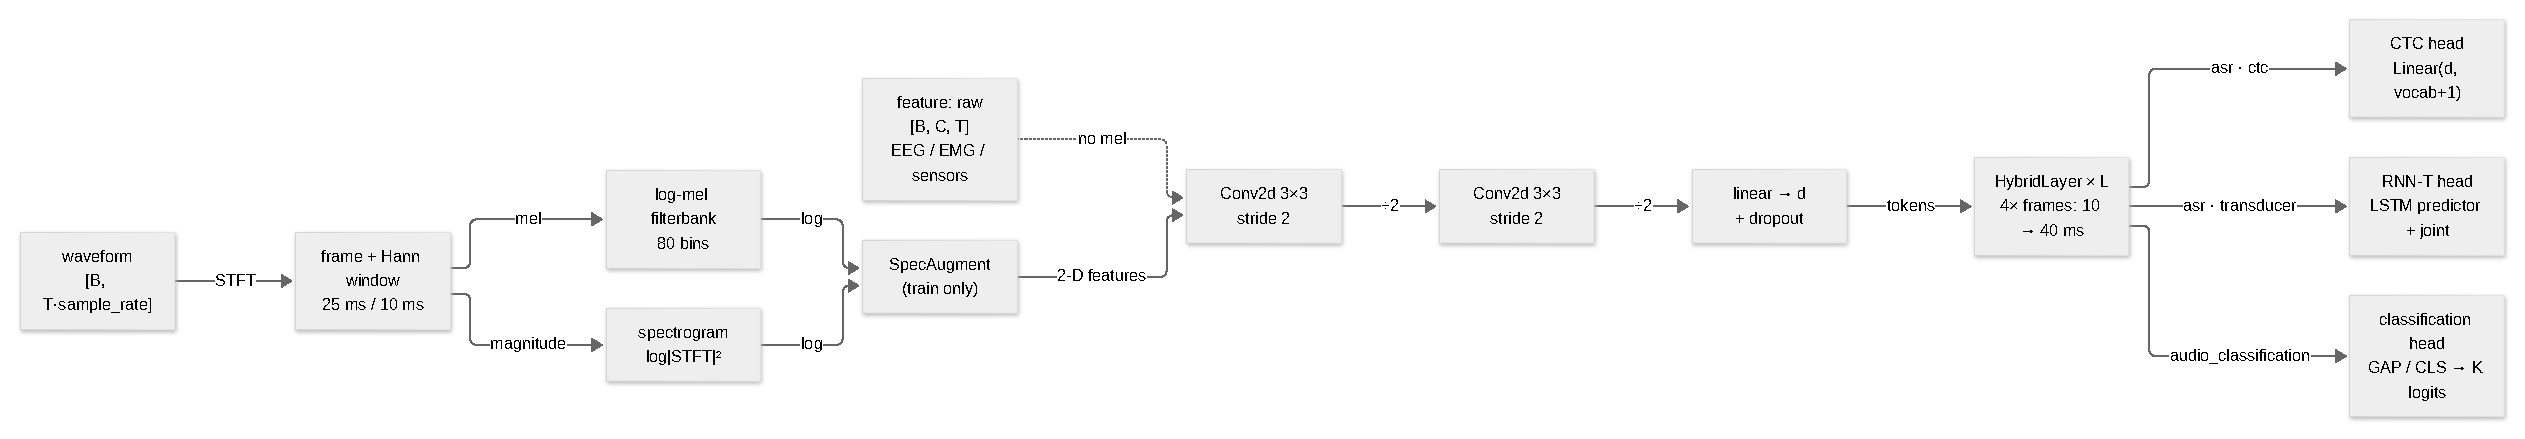
\includegraphics{../paper/figures/audio_frontend.pdf}}
\caption{Flujo de datos del frontend de audio: waveform $\to$ enmarcado 25\,ms/10\,ms $\to$ log-mel de 80 bins (o espectrograma, o tramas multicanal crudas) $\to$ SpecAugment (solo entrenamiento) $\to$ dos etapas Conv2d con stride 2 ($4\times$) $\to$ proyección lineal $\to$ pila \texttt{HybridLayer} $\to$ cabeza CTC, RNN-T o de clasificación.}
\label{fig:audio-frontend}
\end{figure}

\subsubsection{Frontend de Audio}

El módulo frontend convierte un lote de formas de onda $w \in \mathbb{R}^{B \times T}$ (o un lote de clips multicanal $w \in \mathbb{R}^{B \times C \times T}$ en modo \texttt{raw}) en un mapa de características:

\begin{enumerate}[leftmargin=*]
    \item \textbf{Enmarcado:} la forma de onda se corta en ventanas solapadas de \texttt{window\_ms} $=25$\,ms cada \texttt{stride\_ms} $=10$\,ms, con ventana de Hann, a \texttt{sample\_rate} $=16000$\,Hz. A la tasa de referencia esto produce tramas de 400 muestras con salto de 160, es decir, 100 tramas por segundo.
    \item \textbf{Representación espectral} (\texttt{audio.feature}):
    \begin{itemize}[leftmargin=*]
        \item \texttt{logmel} (por defecto): banco de filtros mel de $80$ bins (Ecuación~\ref{eq:audio-mel}) seguido de compresión logarítmica;
        \item \texttt{spectrogram}: $\log|\mathrm{STFT}(w)|^2$ sin proyección mel;
        \item \texttt{raw}: sin transformada espectral; el clip se entrega como mapa $C \times T$ (Sección~\ref{sec:annex-18-eeg}).
    \end{itemize}
    \item \textbf{SpecAugment} \citep{Park2019}: se enmascaran $F$ canales de frecuencia por clip y hasta \texttt{time\_masks} bandas temporales de ancho máximo $p_S \cdot T$, ambas con relleno de ceros (solo entrenamiento).
\end{enumerate}

El banco de filtros mel es
\begin{equation}
M_k(f) = \max\Big(0,\ \min\Big(\tfrac{f-f_{k-1}}{f_k-f_{k-1}},\ \tfrac{f_{k+1}-f}{f_{k+1}-f_k}\Big)\Big),
\label{eq:audio-filterbank}
\end{equation}
para $K = 80$ filtros triangulares espaciados en la escala mel, $\mathrm{mel}(f) = 2595 \log_{10}(1 + f/700)$, y la característica log-mel es
\begin{equation}
x_k = \log\Big(\sum_{f} M_k(f)\,|X(f)|^2 + \epsilon\Big).
\label{eq:audio-mel}
\end{equation}
Cuando \texttt{torchaudio} es importable, el frontend usa \texttt{torchaudio.transforms.MelSpectrogram} para la Ecuación~\ref{eq:audio-mel}; en caso contrario recurre a una implementación en PyTorch puro construida sobre \texttt{torch.stft} y una matriz de filtros en caché. Ambas rutas son numéricamente equivalentes salvo la convención del banco de filtros (espaciado mel HTK vs.\ Slaney), y la ruta en PyTorch puro es la que mantiene la CI solo-CPU libre del extra opcional \texttt{audio}.

\subsubsection{Submuestreo Convolucional}

Dos etapas convolucionales reducen la tasa de tramas $4\times$ (10\,ms $\to$ 40\,ms), que es lo que convierte un utterance de 30 segundos en una secuencia de $\sim$750 tokens en lugar de 3000:
\begin{equation}
F = \mathrm{Dropout}\Big(W_p\,\mathrm{Conv2d}_{3\times3,\,s=2}\big(\mathrm{Conv2d}_{3\times3,\,s=2}(X)\big)\Big),
\qquad W_p \in \mathbb{R}^{d \times d_c},
\label{eq:audio-subsampling}
\end{equation}
donde $X$ es el mapa de características $\texttt{n\_mels} \times T'$ con \texttt{conv\_channels} canales tras la primera etapa, y $W_p$ proyecta los canales aplanados al ancho del modelo $d$. Ambas etapas son fijas, con kernels $3\times3$ y stride 2; \texttt{audio.conv\_channels} (32) fija el ancho de canales de la primera etapa y \texttt{audio.n\_fft} (400) el tamaño de la STFT.

\subsubsection{Modo Encoder Forzado y la Pila HybridLayer}

\texttt{frankenstein\_audio} fuerza \texttt{mode: encoder}, exactamente como \texttt{frankenstein\_vit}: las tareas de audio son bidireccionales (un encoder CTC o transducer debe ver tramas pasadas y futuras), y el padding convolucional del Conformer es simétrico en modo encoder. La clase refleja el patrón envoltorio del ViT---frontend, pila de \texttt{HybridLayer}, cabeza de tarea---y su bucle de capas conserva los mismos hooks, de modo que AttnRes, mHC, Hyperloop, profundidad en bucle, MoE, Mixture-of-Depths y BitNet funcionan sin código específico de audio. Las cabezas de tarea se construyen tras la normalización final:

\begin{itemize}[leftmargin=*]
    \item \textbf{CTC:} $\mathrm{Linear}(d, V+1)$ sobre la secuencia de tramas, donde la clase extra es el blank.
    \item \textbf{RNN-T:} una red de predicción LSTM de una capa sobre las etiquetas no-blank previas (\texttt{audio.asr\_decoder\_dim}, \texttt{asr\_decoder\_layers}, \texttt{asr\_decoder\_dropout}), y una red conjunta $z_{t,u} = \tanh(W_e h_t + W_p h_u + b)$, $\mathrm{logits}_{t,u} = W_o z_{t,u}$.
    \item \textbf{Clasificación:} un vector agrupado (global average pooling, o un token \texttt{[CLS]} aprendido antepuesto a la secuencia de tramas, según \texttt{pooling\_mode}) proyectado a \texttt{num\_classes} logits.
\end{itemize}

\subsection{Reconocimiento Automático de Voz}

\subsubsection{CTC}

La clasificación temporal conexionista \citep{Graves2006ctc} marginaliza sobre todas las alineaciones a nivel de trama que colapsan a la secuencia objetivo $y$ bajo el mapa muchos-a-uno $\mathcal{B}$ (fusionar repeticiones, borrar blanks):
\begin{equation}
\mathcal{L}_{\text{CTC}} = -\log \sum_{\pi \in \mathcal{B}^{-1}(y)} \prod_{t=1}^{T} p(\pi_t \mid x),
\label{eq:audio-ctc}
\end{equation}
calculada con la implementación \texttt{ctc\_loss} de \texttt{torch.nn.functional} en espacio logarítmico con \texttt{zero\_infinity=False}, para que las alineaciones imposibles no envenenen el gradiente.

\subsubsection{RNN-Transducer}

La pérdida RNN-T \citep{Graves2012} suma sobre alineaciones de \emph{etiqueta-y-blank} en la retícula $T \times (U+1)$. Con $\alpha_{t,u}$ la log-probabilidad del prefijo $y_{1:u}$ tras $t$ tramas de encoder, la recursión forward es
\begin{equation}
\alpha_{t,u} = \operatorname{logsumexp}\Big(
\underbrace{\alpha_{t-1,u} + \log p(\varnothing \mid t-1, u)}_{\text{avanzar tiempo}},
\;
\underbrace{\alpha_{t,u-1} + \log p(y_u \mid t, u-1)}_{\text{emitir etiqueta}}
\Big),
\label{eq:audio-rnnt}
\end{equation}
con $\alpha_{0,0} = 0$ y $-\infty$ en el resto, $p(\cdot \mid t,u) = \operatorname{softmax}(\mathrm{logits}_{t,u})$, y
\begin{equation}
\mathcal{L}_{\text{RNN-T}} = -\alpha_{T,U}.
\label{eq:audio-rnnt-loss}
\end{equation} La implementación es compatible con autograd en PyTorch puro (programación dinámica en dominio logarítmico sobre la retícula, con el gradiente obtenido por la recursión backward estándar), y toma la ruta rápida \texttt{torchaudio.functional.rnnt\_loss} cuando la dependencia opcional está instalada. La retícula es $O(T \cdot U)$ en memoria, por lo que el predictor se mantiene superficial (\texttt{audio.asr\_decoder\_layers}, por defecto 1) y estrecho (\texttt{audio.asr\_decoder\_dim}, 320 por defecto). La pérdida se selecciona con \texttt{audio.asr\_loss} (\texttt{ctc} por defecto).

\subsubsection{Decodificación y Tasa de Error}

La decodificación CTC voraz toma el argmax por trama, colapsa repeticiones y elimina blanks. La decodificación RNN-T voraz alterna una emisión de etiqueta con un avance de trama hasta que el blank puntúa más alto que la siguiente etiqueta. Ambas se evalúan con la tasa de error de caracteres
\begin{equation}
\mathrm{CER} = \frac{S + D + I}{N},
\label{eq:audio-cer}
\end{equation}
donde $S$, $D$, $I$ son las sustituciones, deleciones e inserciones del alineamiento de Levenshtein contra la transcripción de referencia y $N$ es la longitud de referencia.

\subsection{Clasificación de Audio}

La clasificación reutiliza las convenciones de pooling y cabeza del Vision Transformer (Anexo~\ref{sec:annex-vision}): \texttt{pooling\_mode: cls} antepone un token aprendido y lee la posición 0, \texttt{pooling\_mode: gap} (el valor por defecto) promedia las salidas de las tramas. La cabeza es un $\mathrm{Linear}(d, K)$ inicializado en cero, entrenado con entropía cruzada y el mismo control de suavizado de etiquetas que las tareas de visión. SpecAugment se aplica al mapa de características antes del submuestreo, de modo que aumenta la entrada, nunca la secuencia de tokens.

\subsection{SpecAugment}

Siguiendo a \citet{Park2019} en su configuración ``LibriSpeech basic'', los dos tipos de máscara se aplican de forma independiente por clip:
\begin{equation}
\Delta f \sim \mathcal{U}[0, F], \quad f_0 \sim \mathcal{U}[0, \nu - \Delta f],
\qquad
\Delta t \sim \mathcal{U}[0, p_S \cdot T], \quad t_0 \sim \mathcal{U}[0, T - \Delta t],
\label{eq:audio-specaugment}
\end{equation}
con $F = 27$, \texttt{time\_masks} $= 10$ y $p_S = 0.05$, cada máscara poniendo a cero un rectángulo $\Delta f \times \Delta t$. La \emph{deformación temporal} (time warping), la tercera transformación de SpecAugment, no está implementada: requiere una deformación del eje temporal por muestra que interactúa mal con el bucketing de longitud fija del dataset. El enmascaramiento de frecuencia y de tiempo concentran la mayor parte del beneficio de regularización en las propias ablaciones del paper, y ambos se desactivan en evaluación.

\subsection{Tamaños de Referencia}

\begin{table}[H]
\centering
\small
\begin{tabular}{L{2.3cm}cccccc}
\toprule
\textbf{Variante} & \textbf{Capas} & \textbf{$d$} & \textbf{Cabezas} & \textbf{Kernel} & \textbf{Paráms.} & \textbf{RNN-T $d_{dec}$} \\
\midrule
Conformer-S & 16 & 144 & 4 & 32 & 10.3M & 320 \\
Conformer-M & 17 & 256 & 4 & 32 & 30.7M & 640 \\
Conformer-L & 17 & 512 & 8 & 32 & 118.8M & 640 \\
\bottomrule
\end{tabular}
\caption{Tamaños de referencia del Conformer de \citet{Gulati2020} (Tabla~1), que siguen los presets de ejemplo. El ancho del decoder RNN-T solo se usa cuando \texttt{audio.asr\_loss: transducer}.}
\label{tab:audio-sizes}
\end{table}

\subsection{Configuraciones de Ejemplo}

Los ejemplos de ASR usan \texttt{astroza/chilean-jokes-festival-de-vina} (audio en español a 16\,kHz con transcripciones, 50 filas), un dataset lo bastante pequeño para ejecutarse de extremo a extremo en CPU como prueba de humo. El ejemplo de clasificación recurre al \texttt{DummyAudioDataset} sintético cuando no hay dataset accesible.

\begin{verbatim}
model_class: frankenstein_audio
model:
  dims: {hidden_size: 144, num_layers: 16, num_heads: 4}
  dims.layer_pattern: [conformer_attn, ...]   # 16 entradas
  attention.conformer: {kernel_size: 32, macaron: true, conv_norm: batch}
audio:
  feature: logmel
  sample_rate: 16000
  n_mels: 80
  window_ms: 25
  stride_ms: 10
  n_fft: 400
  conv_channels: 32
  asr_loss: ctc          # o transducer
  asr_decoder_dim: 320
  asr_decoder_layers: 1
  asr_decoder_dropout: 0.1
audio_dataset:
  dataset_name: astroza/chilean-jokes-festival-de-vina
  split: train
  audio_column: audio
  text_column: text
  spec_augment: {enabled: true, freq_mask_width: 27,
                 time_masks: 10, time_mask_ratio: 0.05}
training:
  task: asr
\end{verbatim}

\subsection{Señales 1-D Genéricas: EEG y Más Allá}
\label{sec:annex-18-eeg}

El frontend no está atado a la voz. Con \texttt{audio.feature: raw}, el banco de filtros mel y SpecAugment se omiten y el clip se trata como un mapa multicanal $C \times T$, con \texttt{audio.in\_channels: C}. Las dos convoluciones con stride 2 actúan entonces como un banco de filtros aprendido sobre el tiempo (y, como efecto secundario, sobre el eje de canales), la proyección lineal produce tokens de ancho $d$, y la pila de \texttt{HybridLayer} ve una secuencia de tramas exactamente como en voz. Esto hace usable la clase, al menos para \textbf{clasificación}, en:

\begin{itemize}[leftmargin=*]
    \item \textbf{EEG:} $C$ electrodos $\times$ $T$ muestras por época, etiquetadas con un estado cognitivo, fase de sueño o patología; los electrodos juegan el papel de los canales mel.
    \item \textbf{EMG / ECG / EDA:} uno o pocos canales, etiquetados con gesto, actividad o clase de anomalía.
    \item \textbf{Acelerómetro / IMU:} $C \in \{3, 6, 9\}$ ejes, etiquetados con actividad o estado del dispositivo.
    \item \textbf{Sensores industriales y ambientales:} trazas de vibración, presión o emisión acústica, etiquetadas por ventana.
\end{itemize}

\paragraph{Qué se conserva.} Todo lo que está aguas abajo del frontend: los 45 mezcladores (Conformer es un buen valor por defecto porque su rama de convolución coincide con la morfología local de las bioseñales), las 6 normas, AttnRes/mHC/MoE/MoD, los 23 optimizadores, la receta de encoder congelado de \texttt{text\_classification} y las rutas de checkpoint y despliegue. El bucketing por longitud, las máscaras de padding y la evaluación tipo CER son del lado del dataset y no dependen de la modalidad.

\paragraph{Limitaciones.} El modo raw es una comodidad, no un reemplazo de un frontend de dominio:
\begin{enumerate}[leftmargin=*]
    \item \textbf{Submuestreo del eje de canales.} Las dos etapas \texttt{Conv2d} con stride 2 son fijas y reducen a la mitad ambos ejes espaciales, así que un montaje con menos de cuatro canales pierde su eje de canales por completo; mantenga $C \geq 4$ (o proyecte el montaje a un mapa más ancho primero).
    \item \textbf{Sin geometría del montaje.} Las posiciones de los electrodos, los montajes referenciales vs.\ bipolares y las correlaciones inter-canal no se codifican; la convolución ve los canales como una pila sin orden, a diferencia de los modelos específicos de EEG con priors topográficos o de grafo.
    \item \textbf{Sin prior espectral.} \texttt{logmel} y \texttt{spectrogram} asumen límites de banda y espaciado mel que no aplican por debajo de 20\,Hz ni por encima de 8\,kHz; el modo raw evita el desajuste pero también pierde el sesgo inductivo alineado a la banda.
    \item \textbf{Solo clasificación.} CTC y RNN-T requieren una secuencia objetivo a nivel de token. El etiquetado secuencia-a-secuencia de ventanas de sensores (p.\,ej.\ secuencias de fases de sueño) queda fuera de alcance; use clasificación por ventana y un decodificador posterior.
    \item \textbf{Estadísticas y normalización.} La BatchNorm del módulo de convolución usa estadísticas por lote; en EEG la escala de amplitud varía por sujeto y sesión, por lo que se recomienda normalizar por canal en el dataset en lugar de confiar en el frontend.
    \item \textbf{Supuestos de tasa de muestreo.} \texttt{sample\_rate} se usa para convertir \texttt{window\_ms}/\texttt{stride\_ms} en muestras; para señales crudas ajústelo a la tasa real de adquisición y elija la ventana en milisegundos en consecuencia.
\end{enumerate}

\subsection{Pseudocódigo en PyTorch}

\begin{algorithmic}[1]
\State \textbf{Entrada:} formas de onda $w$, longitudes $\ell$, transcripciones $y$ (ASR) o etiquetas $c$ (clasificación)
\State $F \gets \texttt{frontend}(w)$ \Comment{log-mel / espectrograma / raw, $(B, C, 80, T')$}
\State $F \gets \texttt{spec\_augment}(F)$ \Comment{solo entrenamiento}
\State $F \gets \texttt{conv2d}_{3\times3, s=2}(F)$; \quad $F \gets \texttt{conv2d}_{3\times3, s=2}(F)$
\State $x \gets \texttt{dropout}(\texttt{linear}(F))$ \Comment{tokens $(B, T'/4, d)$}
\State $x \gets x + \texttt{pos\_encoder}(x)$ \Comment{posiciones de trama, no bins mel}
\For{cada \texttt{layer} en \texttt{layers}}
    \State $x \gets \texttt{layer}(x)$ \Comment{\texttt{HybridLayer}, modo encoder forzado}
\EndFor
\State $x \gets \texttt{final\_norm}(x)$
\If{tarea $=$ asr y pérdida $=$ ctc}
    \State $\mathrm{logits} \gets \texttt{ctc\_head}(x)$; \quad $\mathcal{L} \gets \texttt{ctc\_loss}(\log\mathrm{softmax}(\mathrm{logits}), y, \ell/4)$
\ElsIf{tarea $=$ asr y pérdida $=$ transducer}
    \State $h^{pred} \gets \texttt{predictor}(y)$; \quad $\mathrm{logits}_{t,u} \gets \texttt{joint}(x_t, h^{pred}_u)$
    \State $\mathcal{L} \gets \texttt{rnnt\_loss}(\mathrm{logits}, y, \ell/4)$
\Else
    \State $\mathrm{logits} \gets \texttt{class\_head}(\texttt{pool}(x))$; \quad $\mathcal{L} \gets \mathrm{CE}(\mathrm{logits}, c)$
\EndIf
\end{algorithmic}

\subsection{Desviaciones y Notas de Implementación}

\begin{itemize}[leftmargin=*]
    \item \textbf{torchaudio opcional.} El frontend prefiere \texttt{torchaudio.transforms} pero nunca lo requiere; la alternativa en PyTorch puro mantiene la CI solo-CPU y el extra \texttt{cpu} libres de torchaudio (decisión D7 de la guía de arquitectura).
    \item \textbf{Deformación temporal.} No implementada (la Ecuación~\ref{eq:audio-specaugment} cubre solo enmascaramiento de frecuencia y tiempo); es la transformación que el paper usa menos.
    \item \textbf{Predictor superficial.} La red de predicción RNN-T es una sola capa LSTM por defecto (\texttt{audio.asr\_decoder\_layers}), cambiando el predictor más profundo del paper por una retícula $O(T \cdot U)$ que cabe en memoria con los tamaños de lote de referencia.
    \item \textbf{Exportación.} Las exportaciones a HuggingFace y GGUF rechazan explícitamente los artefactos de audio, como hacen con SBERT: no existe un mapeo upstream \texttt{FrankensteinForAudioClassification}. \texttt{deploy --format standard|quantized} funciona sin cambios.
    \item \textbf{Caché.} No hay caché de encoder incremental para audio; ASR consume un utterance completo por forward.
\end{itemize}
